\documentclass[12pt,dvipsnames]{article}

% Packages
%---------------------------------------------------------------------------------------------------
\usepackage[english]{babel}
\usepackage[svgnames]{xcolor}
\usepackage{natbib}
\usepackage{url}
\usepackage[utf8x]{inputenc}
\usepackage{amsmath}
\usepackage{verbatim}
\usepackage{graphicx}
\usepackage{parskip}
\usepackage{hyperref}
\usepackage{fancyhdr}
\usepackage{listings}
\usepackage{vmargin}
\setmarginsrb{2 cm}{1.5 cm}{2 cm}{1.5 cm}{1 cm}{1 cm}{1.5 cm}{1.5 cm}
\usepackage{minted}
\usepackage{hyperref}
\usepackage{float}
\usepackage{etoolbox}
\usepackage{tcolorbox}
\usepackage[
labelfont=sf,
hypcap=false,
format=hang,
width=\columnwidth
]{caption}

%Colors
%---------------------------------------------------------------------------------------------------
\definecolor{bg}{rgb}{0.95,0.95,0.95}
%---------------------------------------------------------------------------------------------------

% New commands
%---------------------------------------------------------------------------------------------------
\makeatletter
\patchcmd{\verbatim@input}{\@verbatim}{\scriptsize\@verbatim}{}{}
\makeatother

% Highlight some code
\newcommand{\Lcode}[1]{\texttt{\color{Blue}{#1}}}

% Shell command highlighting
\newcommand{\scom}[1]{
\vspace{0.2cm}
\begin{tcolorbox}
    \texttt{\color{Blue}{\$ #1}}
\end{tcolorbox}
}
% Multiple shell command highlighting
\newcommand{\mscom}[1]{
\vspace{0.2cm}
\begin{tcolorbox}
    \texttt{\color{Blue}{#1}}
\end{tcolorbox}
}
% Reference to code lines write only the line number
\newcommand{\refcode}[1]{\underline{line #1}}

% Caption for long listing (can be used also for short listing)
\newcommand{\Caption}[1]{\captionof{listing}{#1}}
%---------------------------------------------------------------------------------------------------


%Definition of image path
%---------------------------------------------------------------------------------------------------
\graphicspath{{images/}}
%---------------------------------------------------------------------------------------------------


% Linking and reference style
%---------------------------------------------------------------------------------------------------
\hypersetup{
  colorlinks=true,
  linkcolor=SteelBlue,
  filecolor=IndianRed,
  urlcolor=IndianRed,
  citecolor=LightSlateGray,
  raiselinks=true
}

% Listing style
%---------------------------------------------------------------------------------------------------
\usemintedstyle{perldoc}
\setminted{
frame=lines,
bgcolor=bg,
fontsize=\footnotesize,
baselinestretch=1,
framesep=1mm,
linenos,
breaklines,
tabsize=1
}
%---------------------------------------------------------------------------------------------------




\begin{document}
%%%%%%%%%%%%%%%%%%%%%%%%%%%%%%%%%%%%%%%%%%%%%%%%%%%%%%%%%%%%%%%%%%%%%%%%%%%%%%%%
%%%%%%%%%%%%%%%%%%%%%%%%%%%%%%%%%%%%%%%%%%%%%%%%%%%%%%%%%%%%%%%%%%%%%%%%%%%%%%%%%%%%%%%%%%%
% cose da modificare ogni volta
%%%%%%%%%%%%%%%%%%%%%%%%%%%%%%%%%%%%%%%%%%%%%%%%%%%%%%%%%%%%%%%%%%%%%%%%%%%%%%%%%%%%%%%%%%%

\title{DeSEm project}													% Title
\author{Fabio Baldo}														% Author
\date{10/01/2021}														% Date

%%%%%%%%%%%%%%%%%%%%%%%%%%%%%%%%%%%%%%%%%%%%%%%%%%%%%%%%%%%%%%%%%%%%%%%%%%%%%%%%%%%%%%%%%%%


\makeatletter
\let\thetitle\@title
\let\theauthor\@author
\let\thedate\@date
\makeatother
\pagestyle{fancy}
\fancyhf{}
\rhead{\theauthor}
\lhead{\thetitle}
\cfoot{\thepage}
\newcommand{\mis}[3]{(#1 \pm #2) \ #3}
\newcommand{\misp}[3]{(#1 \#3 \pm #2}


%%%%%%%%%%%%%%%%%%%%%%%%%%%%%%%%%%%%%%%%%%%%%%%%%%%%%%%%%%%%%%%%%%%%%%%%%%%%%%%%%%%%%%%%%

\begin{titlepage}
	
    \begin{center}				
    \textsc{\LARGE HES-SO MSE}\\[2.0 cm]						% University Name
    
        \makebox[\textwidth]{
\includegraphics[width=\textwidth]{images/HES-SO-Haute-Ecole-Specialisee-de-Suisse-occidentale_ng_image_full.png}} % University Logo
        \vspace*{2.00 cm}
    
	\textsc{\Large Design of communicative embedded systems}\\[0.30 cm]		% Course Code
	\textsc{\Large S1-2021 }\\[0.5 cm]		%Anno accademico
	\textsc{\Large  }\\[0.5 cm] % Nome del Professore
	\rule{\linewidth}{0.2 mm} \\[0.4 cm]
	{ \huge \bfseries \thetitle \\ \small \thedate}\\
	\rule{\linewidth}{0.2 mm} \\[1.5 cm]
	
    	\begin{center}
    	    Fabio Baldo
    	\end{center}
    	
	\end{center}
\end{titlepage}

%%%%%%%%%%%%%%%%%%%%%%%%%%%%%%%%%%%%%%%%%%%%%%%%%%%%%%%%%%%%%%%%%%%%%%%%%%%%%%%%

\tableofcontents

%\renewcommand\listoflistingscaption{List of source codes}
%\listoflistings
\newpage

%%%%%%%%%%%%%%%%%%%%%%%%%%%%%%%%%%%%%%%%%%%%%%%%%%%%%%%%%%%%%%%%%%%%%%%%%%%%%%%%
\section{Diagrams}

\subsection{DeseNET protocol documentation}

\begin{figure}[H]
	\centering
	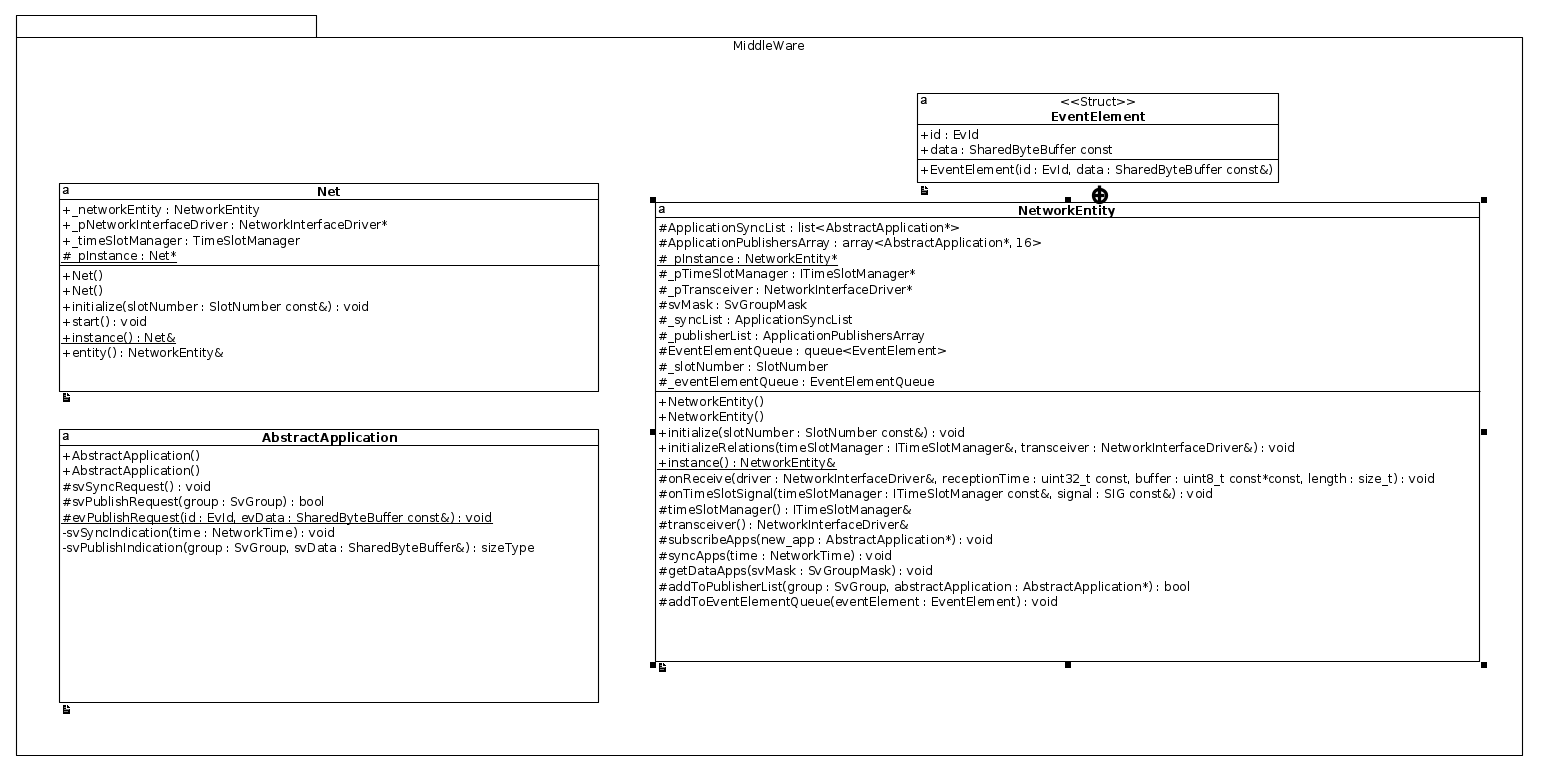
\includegraphics[width=\linewidth]{images/sensor_middleWare.png}
	\caption{Class diagram of the sensor middleware}
	\label{fig:sensor_middleware}
\end{figure}

\begin{figure}[H]
	\centering
	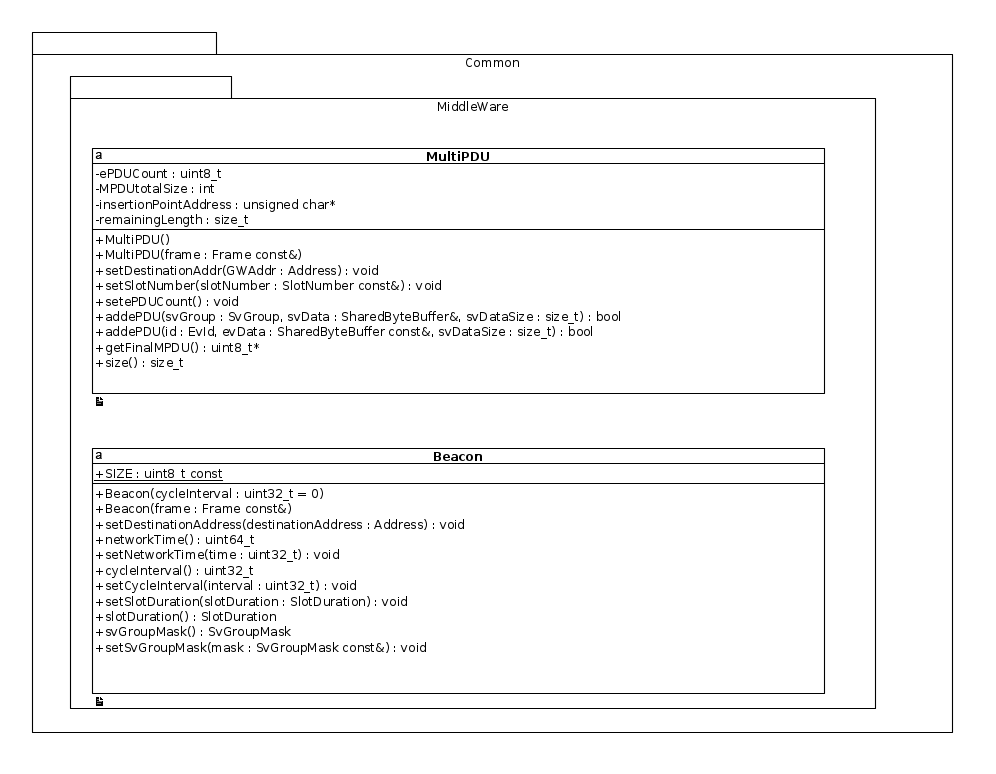
\includegraphics[width=\linewidth]{images/common_MultiPDU_Beacon.png}
	\caption{Class diagram of the two main classes of the Common middleware}
	\label{fig:common_middleware}
\end{figure}

\begin{figure}[H]
	\centering
	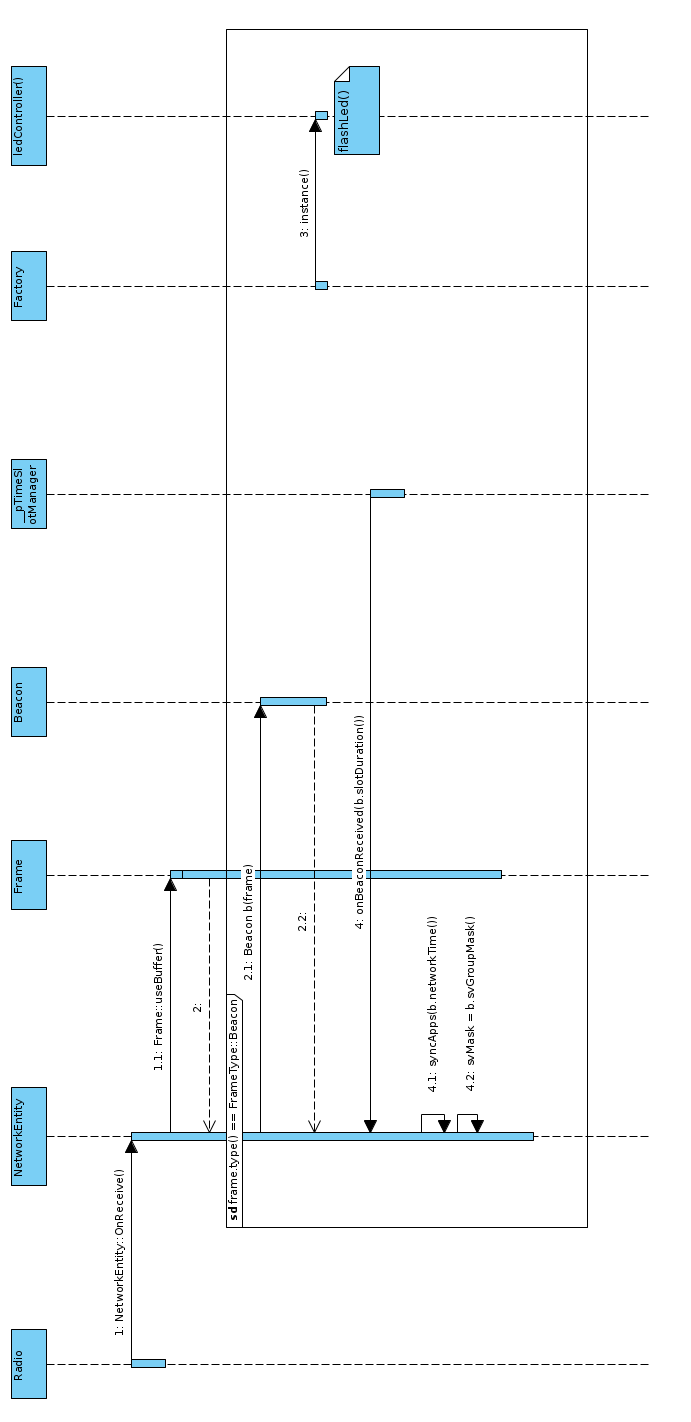
\includegraphics[height=\textheight]{images/onReceive_rotated.png}
	\caption{Action diagram of the function onReceive called when a Beacon is received}
	\label{fig:onReceive}
\end{figure}

\begin{figure}[H]
	\centering
	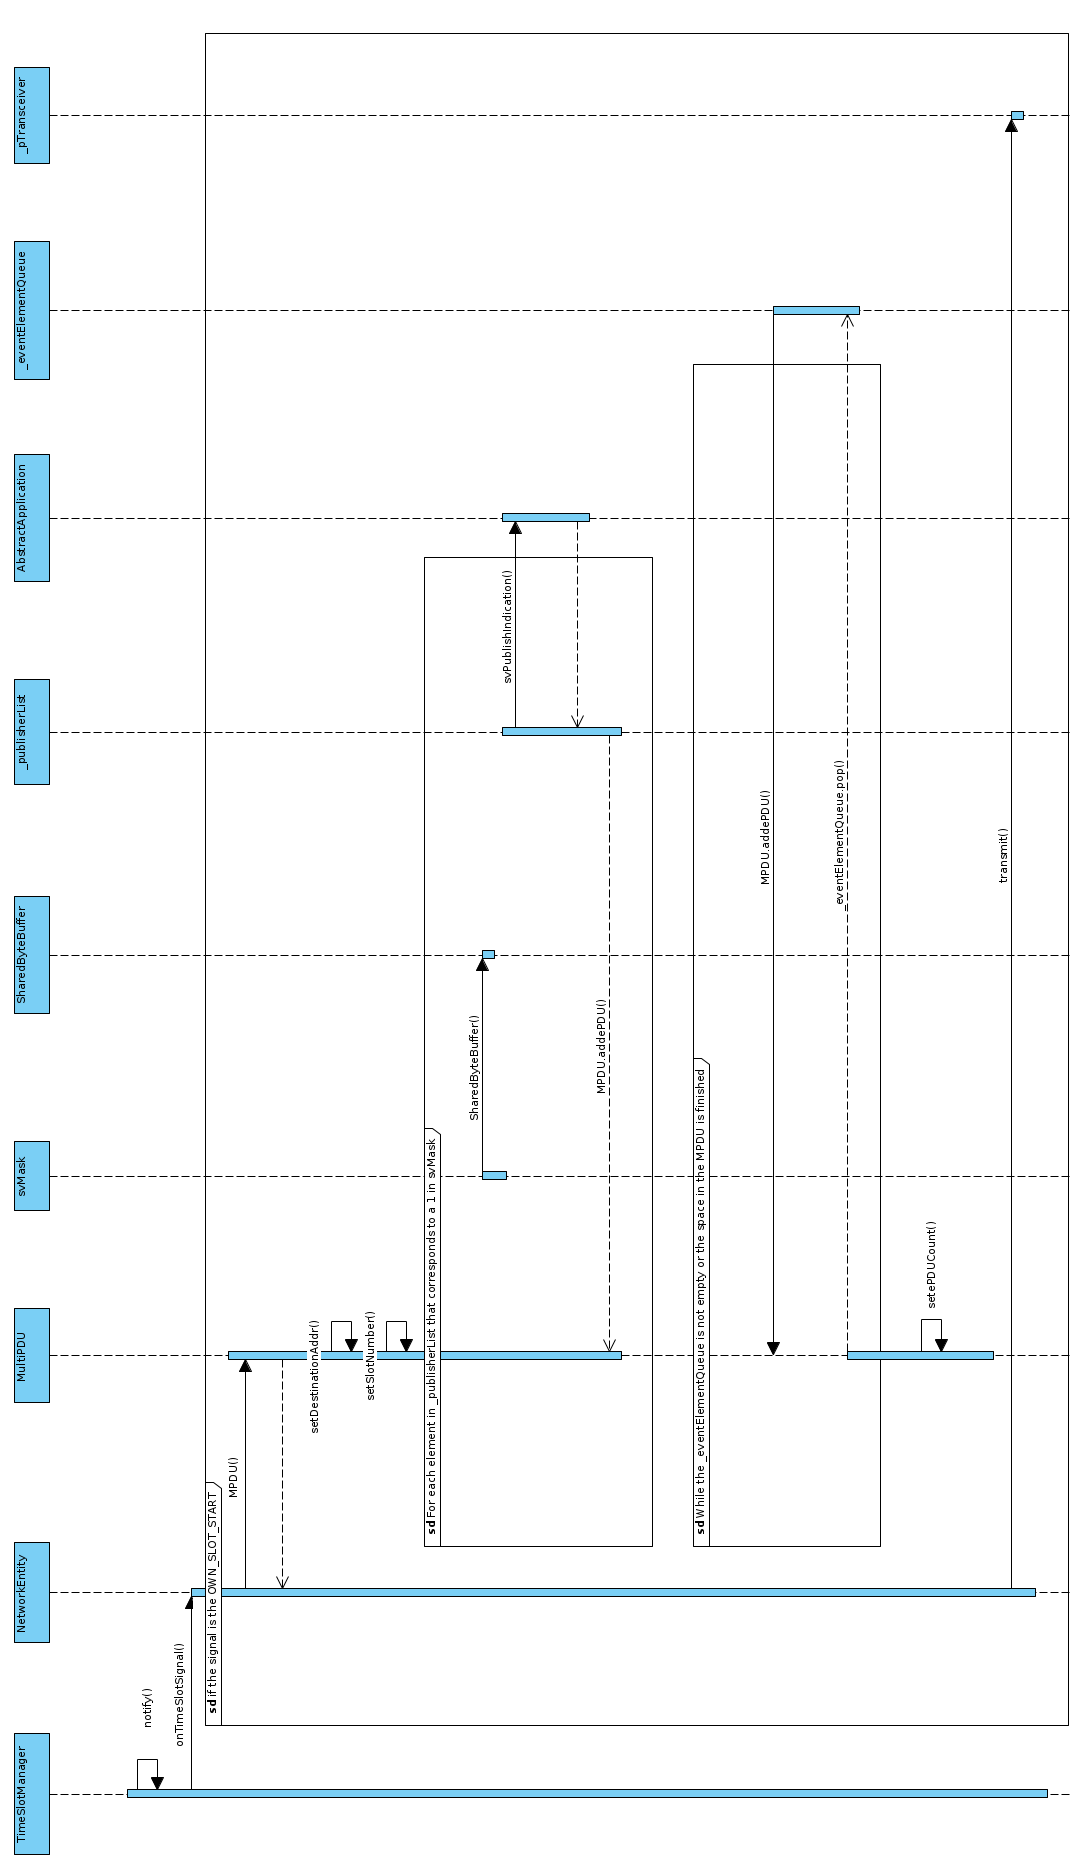
\includegraphics[height=\textheight]{images/onTimeSlotSignal_rotated.png}
	\caption{Action diagram of the function onTimeSlotSignal called when the timer for the slot runs out}
	\label{fig:onTimeSlotSignal}
\end{figure}

\subsection{Joystick application documentation}

\begin{figure}[H]
	\centering
	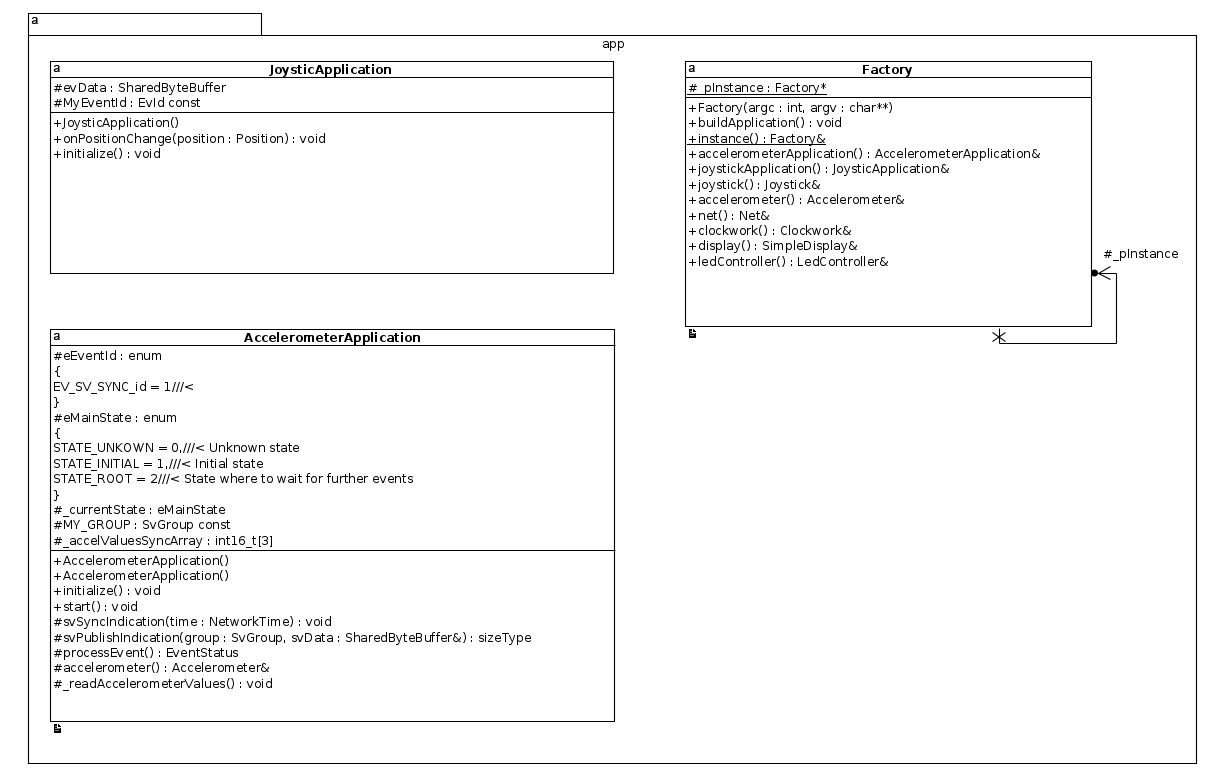
\includegraphics[width=\linewidth]{images/sensors_app.png}
	\caption{Class diagram of the two main classes of the Common middleware}
	\label{fig:common_middleware}
\end{figure}



\section{Tests}

\subsection{DeseNET protocol test}
In order to test the good functioning of the entire deseNET protocol a combination of Tracing and repeated test has been used. For controlling the correctness of the send data, using the Trace class and its method \texttt{outln} the content of the variables has been written to the console both when the data is sampled and send back to the Abstract application and  when the MPDU is formed. The whole buffer hosting the MPDU data has been printed byte per byte in order to make it more readable for understanding its content. This MPDU eventually has been tested against the value shown in the mesh simulator for a final check. In the following listings and images is reported a sample of the testing results.

\subsection{Joystick application test}
Like in the previous section the correctness of the data of the events has been performed by a combination of tracing and repeated test with the double check of the result shown in the mesh simulator. The sample reported in the following images and listing represents a case in which the left button of the joystick has been pressed 3 times.
Unfortunately the function, where the evData are copied into the queue used for building the MPDU, is called two times. Many test have been performed in order to understand from where the error comes.  Testing also the official demo it seams that when only one push is done to the button then two events are send to the GW. In order to try to avoid this problem during the tests of the rest of the application, the values of the push button have been set manually to \texttt{0xAB}. With this simple modification and a small one in the code where only one event over a couple is added to the the MPDU the result has been confirmed to be correct. In the reported example the official demo joystick has been pushed only once. 

\subsection{Results}
Highlighted are the lines of the resulting MPDU containing the values.
\begin{figure}[H]
	\centering
	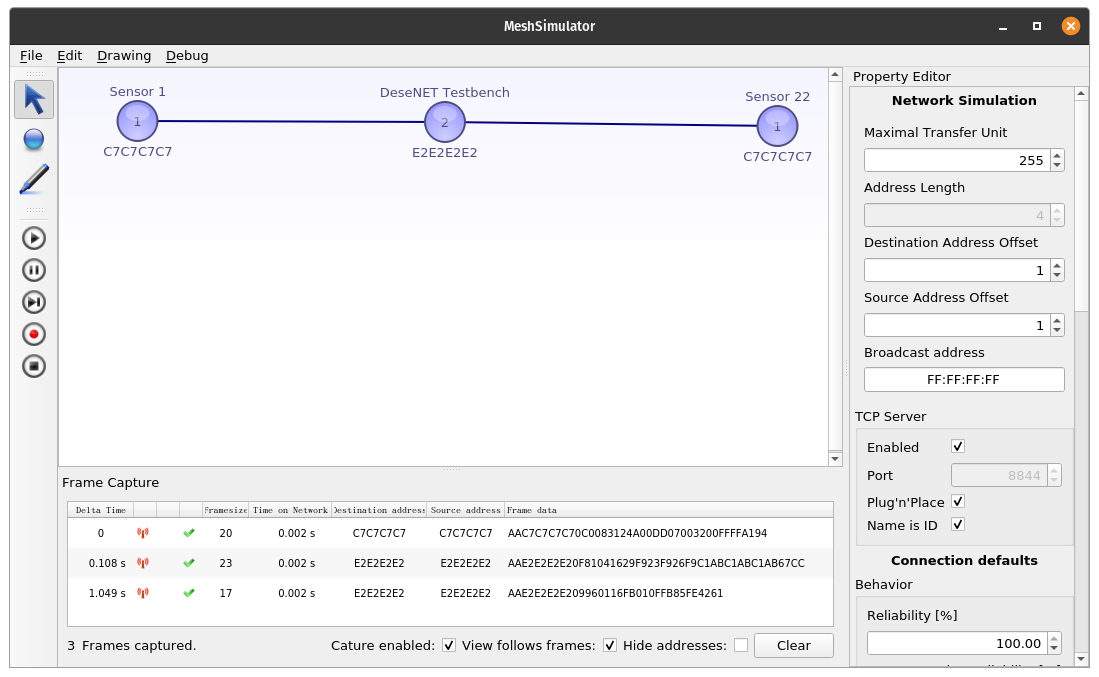
\includegraphics[width=\linewidth]{images/three_clicks_simulation_mesh.png}
	\caption{Screeshot of the simulator window after the MPDU was received from the Sensor back to the GW}
	\label{fig:mesh}
\end{figure}

\begin{figure}[H]
	\centering
	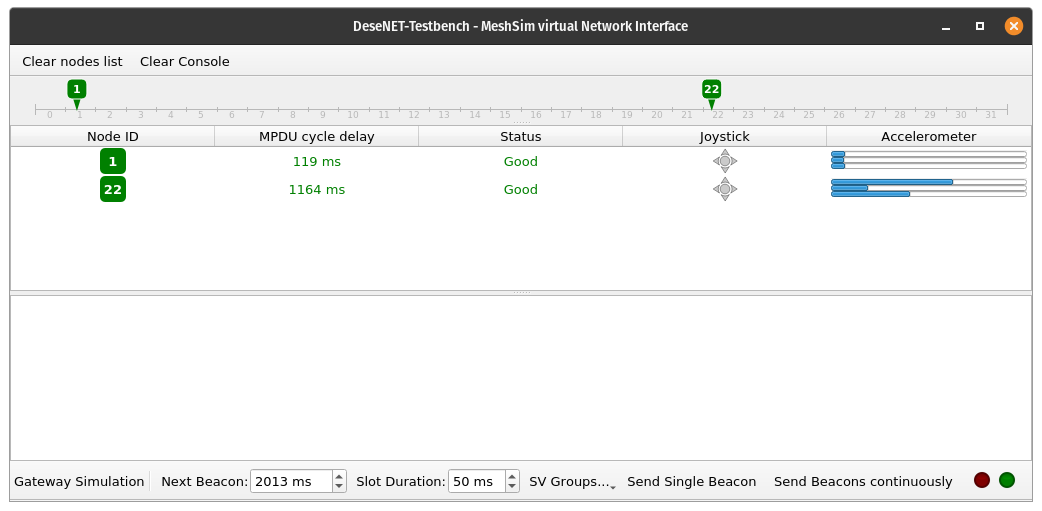
\includegraphics[width=\linewidth]{images/three_clicks_simulation_tb.png}
	\caption{Screeshot of the testbench window after the MPDU was received from the Sensor back to the GW}
	\label{fig:tb}
\end{figure}

\begin{minted}[highlightlines={186-191,193,195,197}]{text}
	AcceApplication data send: 29F923F926F9
	NE_AcceApplication data send: 29F923F926F9
	MPDU before sv-start
	E2
	E2
	E2
	E2
	20
	81
	0
	0
	0
	0
	0
	0
	0
	0
	0
	0
	18
	0
	0
	0
	0
	0
	0
	0
	0
	0
	0
	0
	27
	1
	B5
	1
	E8
	3
	0
	0
	0
	MPDU before sv-end
	MPDU: svData 29F923F926F9
	MPDU: mySVePDU 29F923F926F9
	MPDU after sv-start
	E2
	E2
	E2
	E2
	9
	81
	0
	16
	29
	F9
	23
	F9
	26
	F9
	MPDU after sv-end
	NE_JoysticApplication: Data send: AB
	MPDU before event-start
	E2
	E2
	E2
	E2
	9
	81
	0
	16
	29
	F9
	23
	F9
	26
	F9
	MPDU before event-end
	MPDU after event-start
	E2
	E2
	E2
	E2
	B
	81
	0
	16
	29
	F9
	23
	F9
	26
	F9
	C1
	AB
	MPDU after event-end
	NE_JoysticApplication: Data send: AB
	MPDU before event-start
	E2
	E2
	E2
	E2
	B
	81
	0
	16
	29
	F9
	23
	F9
	26
	F9
	C1
	AB
	MPDU before event-end
	MPDU after event-start
	E2
	E2
	E2
	E2
	D
	81
	0
	16
	29
	F9
	23
	F9
	26
	F9
	C1
	AB
	C1
	AB
	MPDU after event-end
	NE_JoysticApplication: Data send: AB
	MPDU before event-start
	E2
	E2
	E2
	E2
	D
	81
	0
	16
	29
	F9
	23
	F9
	26
	F9
	C1
	AB
	C1
	AB
	MPDU before event-end
	MPDU after event-start
	E2
	E2
	E2
	E2
	F
	81
	0
	16
	29
	F9
	23
	F9
	26
	F9
	C1
	AB
	C1
	AB
	C1
	AB
	MPDU after event-end
	MPDU-start
	E2
	E2
	E2
	E2
	F
	81
	4
	16
	29
	F9
	23
	F9
	26
	F9
	C1
	AB
	C1
	AB
	C1
	AB
	MPDU-end
	
\end{minted}

%%%%%%%%%%%%%%%%%%%%%%%%%%%%%%%%%%%%%%%%%%%%%%%%%%%%%%%%%%%%%%%%%%%%%%%%%%%%%%%%


\end{document}
